

\documentclass{acm_proc_article-sp}
\usepackage{textcomp}
\usepackage{url}
\begin{document}

\title{Who to query? \\A two step querying technique for tracking real-time variant/unknown event distributions }
\numberofauthors{2} %  in this sample file, there are a *total*

\author{
% You can go ahead and credit any number of authors here,
% e.g. one 'row of three' or two rows (consisting of one row of three
% and the second row of one, two or three).
%
% The command \alignauthor (no curly braces needed) should
% precede each author name, affiliation/snail-mail address and
% e-mail address. Additionally, tag each line of
% affiliation/address with \affaddr, and tag the
% e-mail address with \email.
%
% 1st. author
\alignauthor
Mai ElSherief\\
      \affaddr{Dept. of Computer Science }\\
      \affaddr{UC Santa Barbara}\\
     %\affaddr{Santa Barbara, CA}\\
      \email{mayelsherif@cs.ucsb.edu}
% 2nd. author
\alignauthor
Elizabeth Belding\\
     \affaddr{Dept. of Computer Science }\\
      \affaddr{UC Santa Barbara}\\
      %\affaddr{Santa Barbara, CA}\\
      \email{ebelding@cs.ucsb.edu}
}

\maketitle


\begin{abstract}
Some abstract sentences...

\end{abstract}
%\category{H.1.2}{User/Machine Systems}{Human information processing}
%\keywords{Street harassment, Urban analysis, Walkability score, Transit Score, Transit route }


\section{Introduction}
Some introductory sentences...
%In particular, we seek to understand different harassment aspects, such as the location of events and the properties of these locations, so that this information can be used to inform prevention of future events.

\section{Related Work}
- Spatial task distribution (maximizing task assignement)\\
- Applications: emergency scenarios, safety applications, etc. 

\section{Research question and proposed technique}
Given $N$ resources, who should you select to track a real-time phenomenon? 
The answer is that you want to select users with the same distribution as the phenomenon. But what if you do not know the distribution or What if the distribution of the phenomenon is time variant? \cite{adults}

\section{Expermients}
\subsection{Clustered data experminets}
- Begin by pointing out real-life examples of spatially clustered phenomenon and spatial correlation in general.

\begin{figure}[!htb]
\centering
   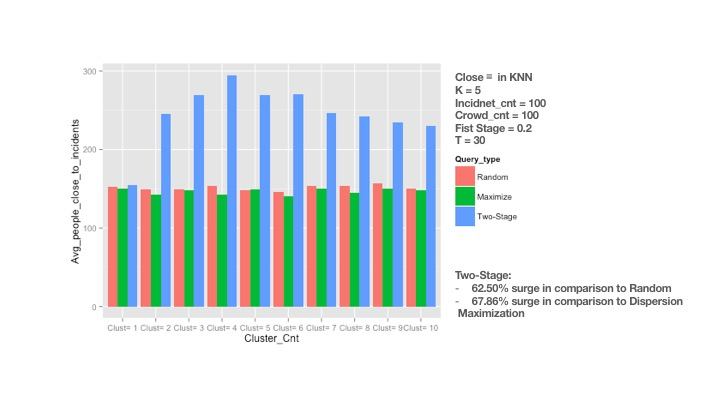
\includegraphics[width=10cm ,height=5.5cm]{figuresPng/FirstStageTwentyPerc}
   \caption{Average number of people close to the incidents when maximizing the dispersion with $20\%$ of available resources. }\label{fig: heatMap}
\end{figure}

\begin{figure}[!htb]
\centering
   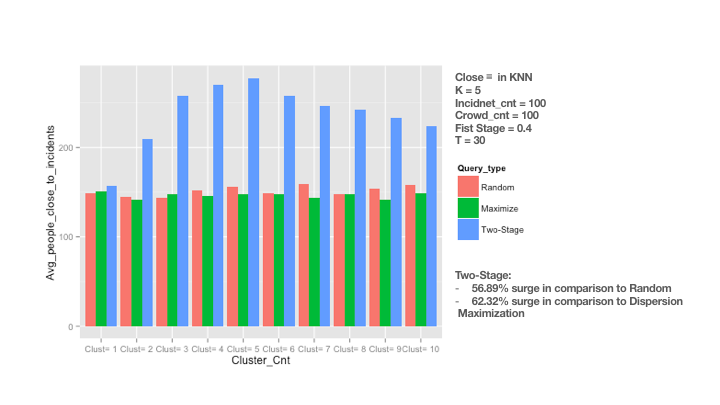
\includegraphics[width=10cm ,height=5.5cm]{figuresPng/FirstStageFortyPerc}
   \caption{Average number of people close to the incidents when maximizing the dispersion with $40\%$ of available resources. }\label{fig: heatMap}
\end{figure}

\begin{figure}[!htb]
\centering
   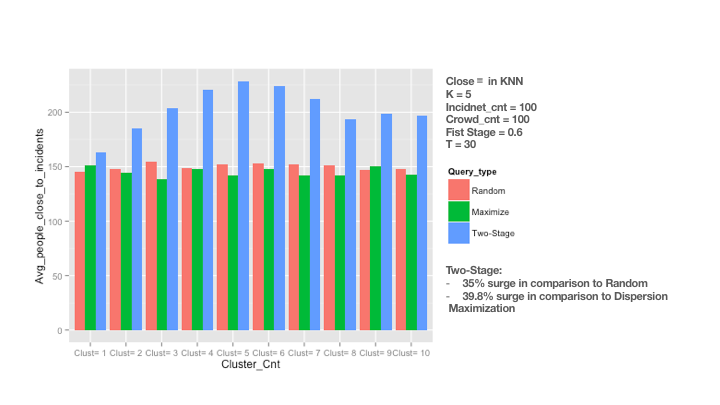
\includegraphics[width=10cm ,height=5.5cm]{figuresPng/FirstStageSixtyPerc}
   \caption{Average number of people close to the incidents when maximizing the dispersion with $60\%$ of available resources. }\label{fig: heatMap}
\end{figure}


\begin{figure}[!htb]
\centering
   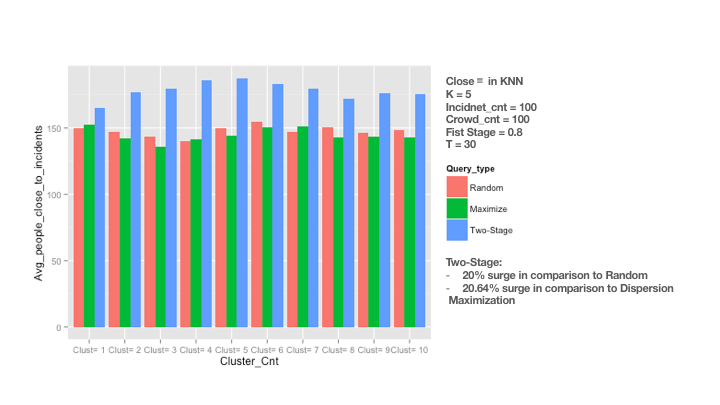
\includegraphics[width=10cm ,height=5.5cm]{figuresPng/FirstStageEightyPerc}
   \caption{Average number of people close to the incidents when maximizing the dispersion with $80\%$ of available resources. }\label{fig: heatMap}
\end{figure}

\begin{figure}[!htb]
\centering
   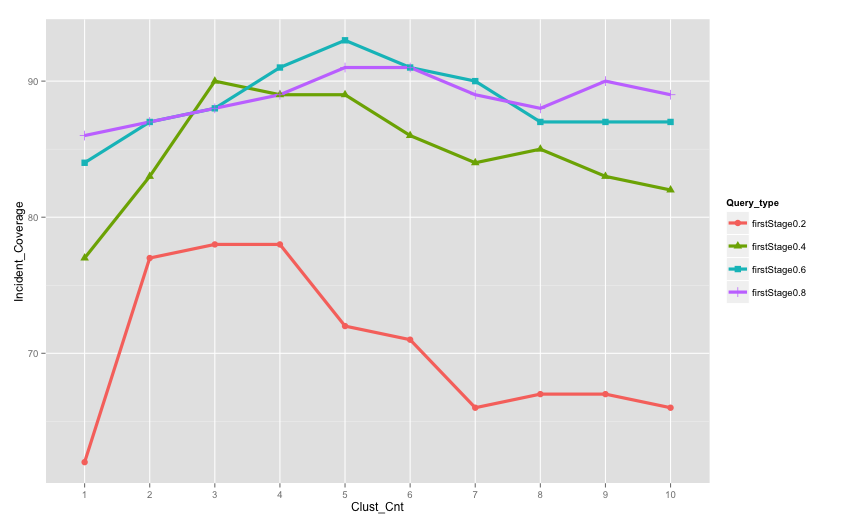
\includegraphics[width=10cm ,height=5.5cm]{figuresPng/Coverage_Result}
   \caption{Number of incidents covered by variations of the two-stage querying technique. }\label{fig: heatMap}
\end{figure}
\subsection{Uniformly distributed data experminets}
\subsection{Case Study: Hollaback harassment data set}
\subsection{Stressing the two stage querying technique (k=1)}

\section{Discussion}
- Our assumptions and limitations...

\section{Conclusions}
In this paper, we introduced.... 

\section{Acknowledgments}

\bibliographystyle{abbrv}
{\footnotesize
\bibliography{sigproc}}  % sigproc.bib is the name of the Bibliography in this case
% You must have a proper ".bib" file
%  and remember to run:
% latex bibtex latex latex
% to resolve all references
%
% ACM needs 'a single self-contained file'!
%
%APPENDICES are optional
%\balancecolumns



\end{document}

